%===============================================================
% Health Assistance System -- Project Documentation
% SE3140 Java Programming 2
%===============================================================
\documentclass[12pt,a4paper]{report}

%---------------------------------------------------------------
% PACKAGES
%---------------------------------------------------------------
\usepackage[a4paper, top=2.5cm, bottom=2.5cm, left=2.8cm, right=2.8cm]{geometry}
\usepackage[T1]{fontenc}
\usepackage[utf8]{inputenc}
%\usepackage{microtype}
\usepackage{xcolor}
\usepackage{graphicx}
\usepackage{eso-pic}
\usepackage{tikz}
\usetikzlibrary{shapes.geometric, arrows.meta, positioning, fit, backgrounds,
                decorations.pathmorphing, shadows, calc}
\usepackage{pgfplots}
\pgfplotsset{compat=1.18}
\usepackage{tcolorbox}
\tcbuselibrary{skins,breakable,theorems,listings}
\usepackage{fancyhdr}
\usepackage{titlesec}
\usepackage{titletoc}
\usepackage{hyperref}
\usepackage{colortbl}
\usepackage{booktabs}
\usepackage{array}
\usepackage{tabularx}
\usepackage{longtable}
\usepackage{multirow}
\usepackage{enumitem}
\usepackage{listings}
\usepackage{mdframed}
\usepackage{float}
\usepackage{caption}
\usepackage{subcaption}
\usepackage{setspace}
\usepackage{parskip}
\usepackage{amsmath}
\usepackage{amssymb}
\usepackage{wrapfig}
\usepackage{afterpage}
\usepackage{pdfpages}
\usepackage{lscape}
\usepackage{rotating}

%---------------------------------------------------------------
% COLOUR PALETTE
%---------------------------------------------------------------
\definecolor{PrimaryBlue}{HTML}{1A3C5E}
\definecolor{AccentTeal}{HTML}{00838F}
\definecolor{AccentGreen}{HTML}{2E7D32}
\definecolor{LightBlue}{HTML}{E3F2FD}
\definecolor{LightTeal}{HTML}{E0F7FA}
\definecolor{LightGreen}{HTML}{E8F5E9}
\definecolor{DarkGray}{HTML}{37474F}
\definecolor{MidGray}{HTML}{607D8B}
\definecolor{LightGray}{HTML}{ECEFF1}
\definecolor{White}{HTML}{FFFFFF}
\definecolor{AlertRed}{HTML}{C62828}
\definecolor{WarnOrange}{HTML}{E65100}
\definecolor{GoldAccent}{HTML}{F9A825}
\definecolor{SectionBar}{HTML}{00ACC1}

%---------------------------------------------------------------
% HYPERREF SETUP
%---------------------------------------------------------------
\hypersetup{
  colorlinks=true,
  linkcolor=PrimaryBlue,
  urlcolor=AccentTeal,
  citecolor=AccentGreen,
  pdftitle={Health Assistance System -- Project Documentation},
  pdfauthor={SE3140 Java Programming 2},
  pdfsubject={Software Engineering Project},
  bookmarks=true,
  bookmarksopen=true,
  pdfpagemode=UseOutlines
}

%---------------------------------------------------------------
% FONTS  (using standard LaTeX fonts)
%---------------------------------------------------------------

%---------------------------------------------------------------
% CHAPTER / SECTION TITLE STYLES
%---------------------------------------------------------------
\newcommand{\chapterbox}[1]{%
  \begin{tcolorbox}[
    colback=PrimaryBlue,colframe=PrimaryBlue,
    arc=4pt,boxrule=0pt,
    left=14pt,right=14pt,top=18pt,bottom=18pt,
    enhanced,shadow={2mm}{-2mm}{0mm}{black!30}
  ]
  \color{White}\huge\bfseries\MakeUppercase{#1}%
  \end{tcolorbox}%
}
\titleformat{\chapter}[display]
  {\normalfont\huge\bfseries\color{White}}
  {}
  {0pt}
  {\chapterbox}
\titlespacing*{\chapter}{0pt}{-20pt}{20pt}

\titleformat{\section}
  {\normalfont\Large\bfseries\color{PrimaryBlue}}
  {\color{AccentTeal}\thesection}
  {0.8em}
  {}
  [\vspace{-4pt}{\color{AccentTeal}\rule{\linewidth}{1.5pt}}]
\titlespacing*{\section}{0pt}{18pt}{8pt}

\titleformat{\subsection}
  {\normalfont\large\bfseries\color{DarkGray}}
  {\color{AccentGreen}\thesubsection}
  {0.7em}
  {}
  [\vspace{-2pt}{\color{LightGray}\rule{\linewidth}{0.8pt}}]
\titlespacing*{\subsection}{0pt}{12pt}{6pt}

\titleformat{\subsubsection}
  {\normalfont\normalsize\bfseries\color{MidGray}}
  {\thesubsubsection}
  {0.6em}
  {}

%---------------------------------------------------------------
% TABLE OF CONTENTS STYLE
%---------------------------------------------------------------
\titlecontents{chapter}[0em]
  {\addvspace{8pt}\bfseries\color{PrimaryBlue}}
  {\contentslabel{1.5em}}
  {\hspace*{-1.5em}}
  {\hfill\color{PrimaryBlue}\contentspage}
\titlecontents{section}[2.2em]
  {\addvspace{2pt}\small\color{DarkGray}}
  {\contentslabel{2em}}
  {\hspace*{-2em}}
  {\titlerule*[0.5em]{.}\contentspage}
\titlecontents{subsection}[4.5em]
  {\addvspace{1pt}\footnotesize\color{MidGray}}
  {\contentslabel{2.5em}}
  {\hspace*{-2.5em}}
  {\titlerule*[0.4em]{.}\contentspage}

%---------------------------------------------------------------
% HEADER / FOOTER
%---------------------------------------------------------------
\pagestyle{fancy}
% Ensure sufficient head height for fancyhdr decorative header
\setlength{\headheight}{15pt}
\fancyhf{}
\renewcommand{\headrulewidth}{0pt}
\fancyhead[L]{%
  
\begin{tikzpicture}[remember picture,overlay]
    \fill[PrimaryBlue] (0,0) rectangle (\textwidth+2cm,0.7cm);
    \node[anchor=west,text=White,font=\small\sffamily] at (0.1cm,0.35cm)
      {\textbf{Health Assistance System}};
    \node[anchor=east,text=White,font=\small\sffamily] at (\textwidth+1.8cm,0.35cm)
      {\leftmark};
  \end{tikzpicture}
}
\fancyfoot[C]{%
  \begin{tikzpicture}[remember picture,overlay]
    \fill[LightGray] (-1.4cm,-0.5cm) rectangle (\textwidth+1.4cm,0.05cm);
    \node[font=\footnotesize\color{MidGray}] at (\textwidth/2,-0.22cm)
      {\thepage};
  \end{tikzpicture}
}
\fancypagestyle{plain}{
  \fancyhf{}
  \fancyfoot[C]{\footnotesize\color{MidGray}\thepage}
  \renewcommand{\headrulewidth}{0pt}
}

%---------------------------------------------------------------
% TCOLORBOX STYLES
%---------------------------------------------------------------
\tcbset{
  infobox/.style={
    colback=LightBlue, colframe=PrimaryBlue,
    arc=4pt, boxrule=1pt,
    left=8pt, right=8pt, top=6pt, bottom=6pt,
    fonttitle=\bfseries\color{PrimaryBlue}
  },
  warnbox/.style={
    colback=LightTeal, colframe=AccentTeal,
    arc=4pt, boxrule=1pt,
    left=8pt, right=8pt, top=6pt, bottom=6pt,
    fonttitle=\bfseries\color{AccentTeal}
  },
  successbox/.style={
    colback=LightGreen, colframe=AccentGreen,
    arc=4pt, boxrule=1pt,
    left=8pt, right=8pt, top=6pt, bottom=6pt,
    fonttitle=\bfseries\color{AccentGreen}
  },
  reqbox/.style={
    enhanced, breakable,
    colback=LightGray, colframe=MidGray,
    arc=3pt, boxrule=0.5pt,
    left=10pt, right=10pt, top=8pt, bottom=8pt
  },
  screenshotbox/.style={
    colback=DarkGray!10, colframe=DarkGray,
    arc=4pt, boxrule=1pt,
    left=6pt, right=6pt, top=6pt, bottom=6pt,
    fonttitle=\bfseries\small
  }
}

%---------------------------------------------------------------
% LISTINGS (code)
%---------------------------------------------------------------
\lstset{
  basicstyle=\ttfamily\small,
  keywordstyle=\color{PrimaryBlue}\bfseries,
  commentstyle=\color{MidGray}\itshape,
  stringstyle=\color{AccentGreen},
  breaklines=true,
  frame=single,
  framerule=0.5pt,
  rulecolor=\color{LightGray},
  backgroundcolor=\color{LightGray!50},
  numbers=left,
  numberstyle=\tiny\color{MidGray},
  numbersep=8pt,
  xleftmargin=15pt,
  captionpos=b
}

%---------------------------------------------------------------
% CUSTOM COMMANDS
%---------------------------------------------------------------
\newcommand{\req}[2]{%
  \begin{tcolorbox}[reqbox,title={\small\textbf{#1}}]
    #2
  \end{tcolorbox}
}

\newcommand{\screenshotPlaceholder}[2]{%
  \begin{tcolorbox}[screenshotbox, title={Screenshot: #1}]
    \begin{center}
      \begin{tikzpicture}
        \fill[White] (0,0) rectangle (12cm,6cm);
        \draw[dashed, MidGray, line width=1pt] (0,0) rectangle (12cm,6cm);
        \node[font=\Large\color{MidGray}] at (6cm,3.5cm) {\textbf{[Screenshot Placeholder]}};
        \node[font=\small\color{MidGray}] at (6cm,2.8cm) {#2};
        \node[font=\footnotesize\color{LightGray!80!MidGray}] at (6cm,2.2cm)
          {Replace this box with actual application screenshot};
        \draw[MidGray, line width=0.5pt] (1cm,1cm) -- (11cm,1cm);
        \draw[MidGray, line width=0.5pt] (6cm,0.4cm) -- (6cm,1.6cm);
      \end{tikzpicture}
    \end{center}
  \end{tcolorbox}%
}

\newcommand{\umlPlaceholder}[2]{%
  \begin{tcolorbox}[screenshotbox, title={UML Diagram: #1}]
    \begin{center}
      \begin{tikzpicture}
        \fill[White!95!PrimaryBlue] (0,0) rectangle (13cm,7cm);
        \draw[dashed, PrimaryBlue!50, line width=1pt] (0,0) rectangle (13cm,7cm);
        \node[font=\large\color{PrimaryBlue}] at (6.5cm,4cm) {\textbf{#1}};
        \node[font=\small\color{MidGray}] at (6.5cm,3.2cm) {#2};
      \end{tikzpicture}
    \end{center}
  \end{tcolorbox}%
}

% Coloured table rows
\newcommand{\rowH}{\rowcolor{PrimaryBlue!15}}
\newcommand{\rowE}{\rowcolor{White}}
\newcommand{\rowO}{\rowcolor{LightGray!60}}

%===============================================================
% DOCUMENT BEGIN
%===============================================================
\begin{document}
\setstretch{1.25}

%---------------------------------------------------------------
% COVER PAGE
%---------------------------------------------------------------
\begin{titlepage}
\pagecolor{PrimaryBlue}
\afterpage{\nopagecolor}

\begin{tikzpicture}[remember picture, overlay]
  % Background gradient rectangles
  \fill[AccentTeal!40!PrimaryBlue] (current page.north west)
    rectangle ([yshift=-8cm]current page.north east);
  % Decorative circles
  \fill[White, opacity=0.05] ([xshift=3cm,yshift=-3cm]current page.north east) circle (5cm);
  \fill[AccentTeal, opacity=0.10] ([xshift=-2cm,yshift=-12cm]current page.north east) circle (3cm);
  \fill[White, opacity=0.04] ([xshift=2cm,yshift=4cm]current page.south west) circle (4cm);
  % Bottom bar
  \fill[AccentTeal] (current page.south west) rectangle
    ([yshift=2.5cm]current page.south east);
\end{tikzpicture}

\vspace*{2cm}
\begin{center}

% Logo image
\begin{center}
  
\includegraphics[width=5.0cm]{assets/logo.png}
\end{center}

\vspace{0.6cm}
{\fontsize{42}{48}\selectfont\bfseries\sffamily\color{White}
Health Assistance\\[4pt]System}

\vspace{0.5cm}
{\color{AccentTeal!60!White}\rule{10cm}{1.5pt}}

\vspace{0.4cm}
{\Large\sffamily\color{White!85!PrimaryBlue}
Comprehensive Java Programming Project Documentation}

\vspace{1.8cm}

\begin{tcolorbox}[
  colback=White!10!PrimaryBlue, colframe=White!30!PrimaryBlue,
  arc=6pt, boxrule=1pt,
  width=11cm,
  left=16pt, right=16pt, top=14pt, bottom=14pt
]
\begin{tabular}{@{}ll@{}}
  \color{AccentTeal}\textbf{Course Code:}  & \color{White}SE3140 \\[6pt]
  \color{AccentTeal}\textbf{Course Title:} & \color{White}Java Programming 2 \\[6pt]
  \color{AccentTeal}\textbf{Instructor:}   & \color{White}Mughe Godlove \\[6pt]
  \color{AccentTeal}\textbf{Group Number:} & \color{White}22 \\[6pt]
  \color{AccentTeal}\textbf{GitHub Repo:}  & \color{White}\href{https://github.com/Kynmmarshall/HealthAssistanceSystem}{\underline{HealthAssistanceSystem}} \\[6pt]
  \color{AccentTeal}\textbf{Date:}         & \color{White}05/16/2026 \\
\end{tabular}
\end{tcolorbox}

\vspace{1.4cm}

\begin{tcolorbox}[
  colback=White!5!PrimaryBlue, colframe=White!20!PrimaryBlue,
  arc=4pt, boxrule=0.8pt,
  width=18cm,
  left=20pt, right=20pt, top=18pt, bottom=18pt,
  title={\color{GoldAccent}\Large\textbf{Group Members}},
  attach boxed title to top left={yshift=-2mm, xshift=4mm},
  boxed title style={colback=PrimaryBlue,colframe=GoldAccent,arc=2pt,boxrule=0.8pt}
]
\begin{tabular}{@{}c>{\hspace{1cm}}l>{\hspace{1cm}}l>{\hspace{1cm}}l@{}}
  \color{MidGray!50!White}\normalsize\textbf{SN} &
  \color{White}\normalsize\textbf{Member's Name} &
  \color{White}\normalsize\textbf{Reg. Number} &
  \color{White}\normalsize\textbf{Role} \\[12pt]
  \color{AccentTeal}\large 1 & \color{White!100!PrimaryBlue}\normalsize Kamdeu Yamdjeuson Neil Marshall&
    \color{White!100!PrimaryBlue}\normalsize ICTU20241386 &
    \color{White!100!PrimaryBlue}\normalsize Scrum Master \\[14pt]
  \color{AccentTeal}\large 2 & \color{White!100!PrimaryBlue}\normalsize Lemma Precious &
    \color{White!100!PrimaryBlue}\normalsize ICTU2024 &
    \color{White!100!PrimaryBlue}\normalsize Product Owner \\[2pt]
\end{tabular}
\end{tcolorbox}

\vfill

\begin{tikzpicture}[remember picture, overlay]
  \node[anchor=south, yshift=0.7cm, font=\small\color{White!70!PrimaryBlue}]
    at (current page.south)
    {Java Programming 2 $\cdot$ Software Engineering $\cdot$ Academic Year 2024/2025};
\end{tikzpicture}

\end{center}
\end{titlepage}

%---------------------------------------------------------------
% ABSTRACT
%---------------------------------------------------------------
\chapter*{Abstract}
\addcontentsline{toc}{chapter}{Abstract}

\begin{tcolorbox}[
  enhanced, breakable,
  colback=LightBlue, colframe=PrimaryBlue,
  arc=6pt, boxrule=1.5pt,
  left=16pt, right=16pt, top=14pt, bottom=14pt
]
The \textbf{Health Assistance System} is an innovative, community-driven software platform developed as part of the SE3140 Java Programming 2 course. The system addresses the growing need for accessible, digital healthcare assistance by providing users with tools to manage their personal health data, consult symptom checkers, schedule medical appointments, receive medication reminders, and access curated health information resources --- all from a unified, user-friendly interface.

\medskip
Developed following the Scrum agile methodology, the project progresses through five structured phases: team organization, requirements elicitation, architectural and UML design, implementation, and testing with deployment. The system employs a layered MVC architecture that separates the JavaFX screens, controller logic, DAO access, and database models.

\medskip
This documentation presents the complete lifecycle of the Health Assistance System --- from problem definition and use-case modelling to system architecture, UML diagrams, implementation details, and testing results. It serves as the official project report fulfilling all requirements set forth in the SE3140 project specification.
\end{tcolorbox}

\bigskip
\noindent\textbf{Keywords:} Health Management, Java, Scrum, UML, MVC Architecture, JavaFX Desktop Application, Software Engineering, Community Health

%---------------------------------------------------------------
% TABLE OF CONTENTS
%---------------------------------------------------------------
\tableofcontents
\clearpage

%===============================================================
% CHAPTER 1 -- INTRODUCTION
%===============================================================
\chapter{Introduction}

\section{Brief Overview of the Project}

The \textbf{Health Assistance System} is a full-stack Java-based application designed to provide individuals with intelligent, accessible, and personalised health management tools. The platform bridges the gap between patients and health information by delivering a comprehensive set of features through a clean, responsive user interface. The system enables users to log symptoms, track health metrics, book appointments, and receive smart health recommendations --- empowering communities to make informed health decisions without immediate access to medical professionals.

\begin{tcolorbox}[infobox, title={Project at a Glance}]
\begin{tabular}{@{}lp{9cm}@{}}
  \textbf{Application Type:}   & JavaFX Desktop Application \\[3pt]
  \textbf{Technology Stack:}   & JavaFX, FXML, CSS, JDBC, MySQL \\[3pt]
  \textbf{Architecture:}       & Layered MVC with DAO-based data access \\[3pt]
  \textbf{Methodology:}        & Agile Scrum (6-week sprints) \\[3pt]
  \textbf{Target Deployment:}  & Local Desktop Application Build \\
\end{tabular}
\end{tcolorbox}

\section{Problem Statement}

Access to basic health assistance remains a significant challenge in many communities. Individuals frequently face:
\begin{itemize}[leftmargin=1.5cm]
  \item Long waiting times at healthcare facilities for minor consultations
  \item Lack of organised personal health records and medication tracking
  \item Difficulty in monitoring chronic conditions (blood pressure, glucose, etc.)
  \item Limited access to reliable, contextualised health information
  \item Poor medication adherence due to lack of reminder systems
\end{itemize}

The Health Assistance System directly addresses these pain points by delivering a digital health companion accessible anytime, anywhere.

\section{Objectives and Purpose}

\begin{tcolorbox}[successbox, title={Core Objectives}]
\begin{enumerate}[leftmargin=1.2cm]
  \item Provide a centralised platform for personal health record management
  \item Offer a symptom checker powered by a curated medical knowledge base
  \item Enable online appointment scheduling and management
  \item Deliver medication reminders and adherence tracking
  \item Facilitate access to verified health education resources
  \item Ensure secure, role-based access for patients and healthcare providers
\end{enumerate}
\end{tcolorbox}

\section{Key Features and Innovations}

\begin{table}[H]
\centering
\caption{Key System Features}
\begin{tabularx}{\textwidth}{>{\bfseries\color{PrimaryBlue}}l X}
\toprule
\rowcolor{PrimaryBlue!15}
\textbf{Feature} & \textbf{Description} \\
\midrule
\rowO Role-based Authentication & Secure login with role-specific dashboards (Patient, Doctor, Admin). \\
\rowE Appointment Management & Full CRUD with conflict checks, expiration tracking, and slot reactivation. \\
\rowO Appointment Reminders & Background alerts with JavaFX popups and audio playback (MP3 or system beep). \\
\rowE Health Records & Persistent patient data, medical records, and prescriptions via DAO and MySQL. \\
\rowO Role-based Dashboards & Customised views showing relevant metrics, appointments, and quick actions. \\
\rowE Background Threading & Daemon reminder task with safe JavaFX UI updates via \texttt{Platform.runLater()}. \\\bottomrule
\end{tabularx}
\end{table}


%===============================================================
% CHAPTER 2 -- PROJECT MANAGEMENT (SCRUM)
%===============================================================
\chapter{Project Management (Scrum)}

\section{Team Roles and Responsibilities}

\begin{table}[H]
\centering
\caption{Team Roles and Responsibilities}
\begin{tabularx}{\textwidth}{>{\bfseries}l l X}
\toprule
\rowcolor{PrimaryBlue!15}
\textbf{Member} & \textbf{Role} & \textbf{Responsibilities} \\
\midrule
\rowO Kamdeu Yamdjeuson & Application Logic / Database Dev &
  Sprint facilitation, DAO development, database design, reminder task logic \\
\rowE Lemma Precious & UI / Workflow Dev &
  FXML screens, controller logic, validation, and JavaFX interface implementation \\
\bottomrule
\end{tabularx}
\end{table}

\section{Overview of the Scrum Process}

The project adopted the \textbf{Scrum framework}, organising work into six weekly sprints aligned with the six project phases. Each sprint followed the standard Scrum ceremonies:

\begin{tcolorbox}[warnbox, title={Scrum Ceremonies}]
\begin{description}[leftmargin=2cm, style=nextline]
  \item[Sprint Planning] Conducted at the start of each week to select and estimate backlog items
  \item[Daily Stand-ups] 15-minute synchronisation meetings covering: done / doing / blockers
  \item[Sprint Review] Demonstration of completed features to the instructor / stakeholders
  \item[Sprint Retrospective] Team reflection on process improvement and lessons learned
\end{description}
\end{tcolorbox}

\section{Sprint Planning Summary}

\begin{table}[H]
\centering
\caption{Sprint Plan Overview}
\begin{tabularx}{\textwidth}{c l X l}
\toprule
\rowcolor{PrimaryBlue!15}
\textbf{Sprint} & \textbf{Week} & \textbf{Goal / Deliverables} & \textbf{Status} \\
\midrule
\rowO 1 & Week 1 & Team setup, GitHub repo, project charter & \textcolor{AccentGreen}{\textbf{Done}} \\
\rowE 2 & Week 2 & Requirements elicitation and backlog creation & \textcolor{AccentGreen}{\textbf{Done}} \\
\rowO 3 & Week 3 & HLD architecture, component diagrams & \textcolor{AccentGreen}{\textbf{Done}} \\
\rowE 4 & Week 4 & UML diagrams, core backend implementation & \textcolor{AccentGreen}{\textbf{Done}} \\
\rowO 5 & Week 5 & Frontend development, API integration, module completion & \textcolor{AccentGreen}{\textbf{Done}} \\
\rowE 6 & Week 6 & Testing, deployment, documentation, presentation & \textcolor{AccentGreen}{\textbf{Done}} \\
\bottomrule
\end{tabularx}
\end{table}

\section{Product Backlog}

\begin{longtable}{clp{7cm}cc}
\caption{Product Backlog}\\
\toprule
\rowcolor{PrimaryBlue!15}
\textbf{ID} & \textbf{Epic} & \textbf{User Story} & \textbf{Priority} & \textbf{Pts} \\
\midrule
\endfirsthead
\multicolumn{5}{l}{\footnotesize\textit{(Continued from previous page)}} \\[2pt]
\toprule
\rowcolor{PrimaryBlue!15}
\textbf{ID} & \textbf{Epic} & \textbf{User Story} & \textbf{Priority} & \textbf{Pts} \\
\midrule
\endhead
\midrule
\endfoot
\bottomrule
\endlastfoot
US01 & Authentication & As a user I can register and log in securely & High & 5 \\
\rowO US02 & Profile & As a user I can manage my personal health profile & High & 3 \\
US03 & Symptom Checker & As a user I can enter symptoms and receive possible conditions & High & 8 \\
\rowO US04 & Appointments & As a user I can view available doctors and book appointments & High & 8 \\
US05 & Appointments & As a doctor I can view and manage my appointment schedule & High & 5 \\
\rowO US06 & Medications & As a user I can log medications and set reminders & Medium & 5 \\
US07 & Dashboard & As a user I can view my health metrics on a dashboard & Medium & 5 \\
\rowO US08 & Records & As a user I can upload and view my medical records & Medium & 3 \\
US09 & Library & As a user I can browse health education articles & Low & 3 \\
\rowO US10 & Emergency & As a user I can access emergency contacts quickly & High & 2 \\
US11 & Admin & As an admin I can manage users and system settings & Medium & 5 \\
\rowO US12 & Notifications & As a user I receive medication and appointment reminders & Medium & 5 \\
\end{longtable}


%===============================================================
% CHAPTER 3 -- DESIGN AND ARCHITECTURE
%===============================================================
\chapter{Application Design and Architecture}

\section{Overview of Front-End Design}

\subsection{UI/UX Design Principles}

The Health Assistance System interface adheres to the following design principles:

\begin{itemize}[leftmargin=1.5cm]
  \item \textbf{Simplicity:} Clean, uncluttered layouts reducing cognitive load for health-anxious users
  \item \textbf{Accessibility:} High-contrast colour scheme, readable fonts, and keyboard navigation
  \item \textbf{Consistency:} Uniform component library across all screens (buttons, cards, inputs)
  \item \textbf{Responsive Design:} Adaptive layouts for desktop, tablet, and mobile viewports
  \item \textbf{User Feedback:} Immediate visual confirmation of actions (toasts, progress indicators)
\end{itemize}

%---------------------------------------------------------------
\section{System Architectural Design}
%---------------------------------------------------------------

\subsection{High-Level Architecture Diagram}

\begin{figure}[H]
\centering
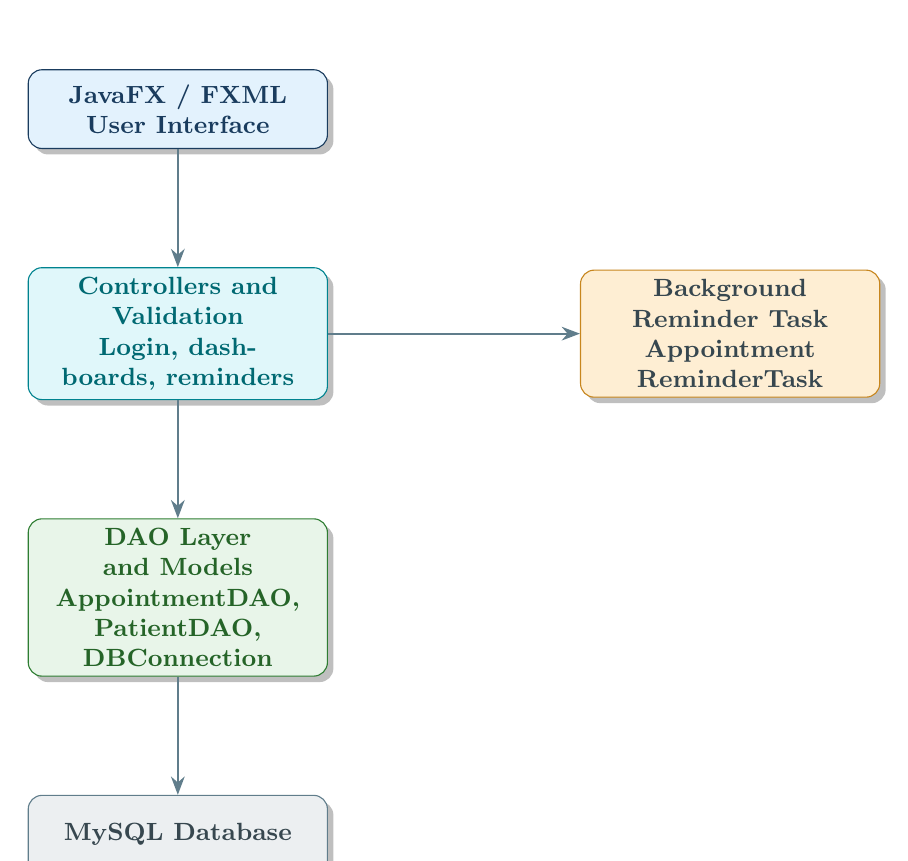
\begin{tikzpicture}[
  node distance=1.5cm and 1.8cm,
  box/.style={rectangle, rounded corners=5pt, minimum width=3.8cm,
    minimum height=1cm, text width=3.4cm, align=center, font=\small\bfseries,
    drop shadow},
  arr/.style={-{Stealth}, thick, color=MidGray}
]

\node[box, fill=LightBlue, draw=PrimaryBlue, text=PrimaryBlue] (ui)
  {JavaFX / FXML User Interface};
\node[box, fill=LightTeal, draw=AccentTeal, text=AccentTeal!80!black,
  below=of ui] (ctrl) {Controllers and Validation\\Login, dashboards, reminders};
\node[box, fill=LightGreen, draw=AccentGreen, text=AccentGreen!80!black,
  below=of ctrl] (dao) {DAO Layer and Models\\AppointmentDAO, PatientDAO, DBConnection};
\node[box, fill=LightGray, draw=MidGray, text=DarkGray,
  below=of dao] (db) {MySQL Database};
\node[box, fill=GoldAccent!20, draw=GoldAccent!80!black, text=DarkGray,
  right=3.2cm of ctrl] (bg) {Background Reminder Task\\Appointment ReminderTask};

% Arrows
\draw[arr] (ui) -- (ctrl);
\draw[arr] (ctrl) -- (dao);
\draw[arr] (dao) -- (db);
\draw[arr] (ctrl) -- (bg);

\end{tikzpicture}
\caption{High-Level System Architecture}
\end{figure}

\subsection{Architecture Description}

The Health Assistance System adopts a \textbf{Layered MVC Architecture} organised into four practical layers:

\begin{description}[leftmargin=2cm, style=nextline]
  \item[Presentation Layer] JavaFX scenes defined with FXML and styled with CSS.
  \item[Controller Layer] Java controller classes handle user actions, validation, and navigation.
  \item[Data Access Layer] DAO classes and \texttt{DBConnection} manage JDBC queries and database operations.
  \item[Data Layer] MySQL stores users, appointments, doctors, patients, and health records.
\end{description}

\subsection{Non-Functional Requirements from Architecture}

\begin{table}[H]
\centering
\caption{Non-Functional Requirements}
\begin{tabularx}{\textwidth}{l X l}
\toprule
\rowcolor{PrimaryBlue!15}
\textbf{NFR} & \textbf{How Architecture Addresses It} & \textbf{Target} \\
\midrule
\rowO Security & Role-based login validation and form checks & Good \\
Scalability & Modular controllers and DAOs make features easy to extend & Good \\
\rowO Performance & Lightweight desktop app with direct JDBC access & Fast response \\
Availability & Runs locally when the application is open & High during use \\
\rowO Maintainability & MVC separation and reusable DAO classes & High \\
Data Integrity & SQL constraints and input validation protect records & High \\
\bottomrule
\end{tabularx}
\end{table}

%---------------------------------------------------------------
\section{Low-Level Design -- UML Diagrams}
%---------------------------------------------------------------

\subsection{Use Case Diagram}

\begin{figure}[H]
\centering
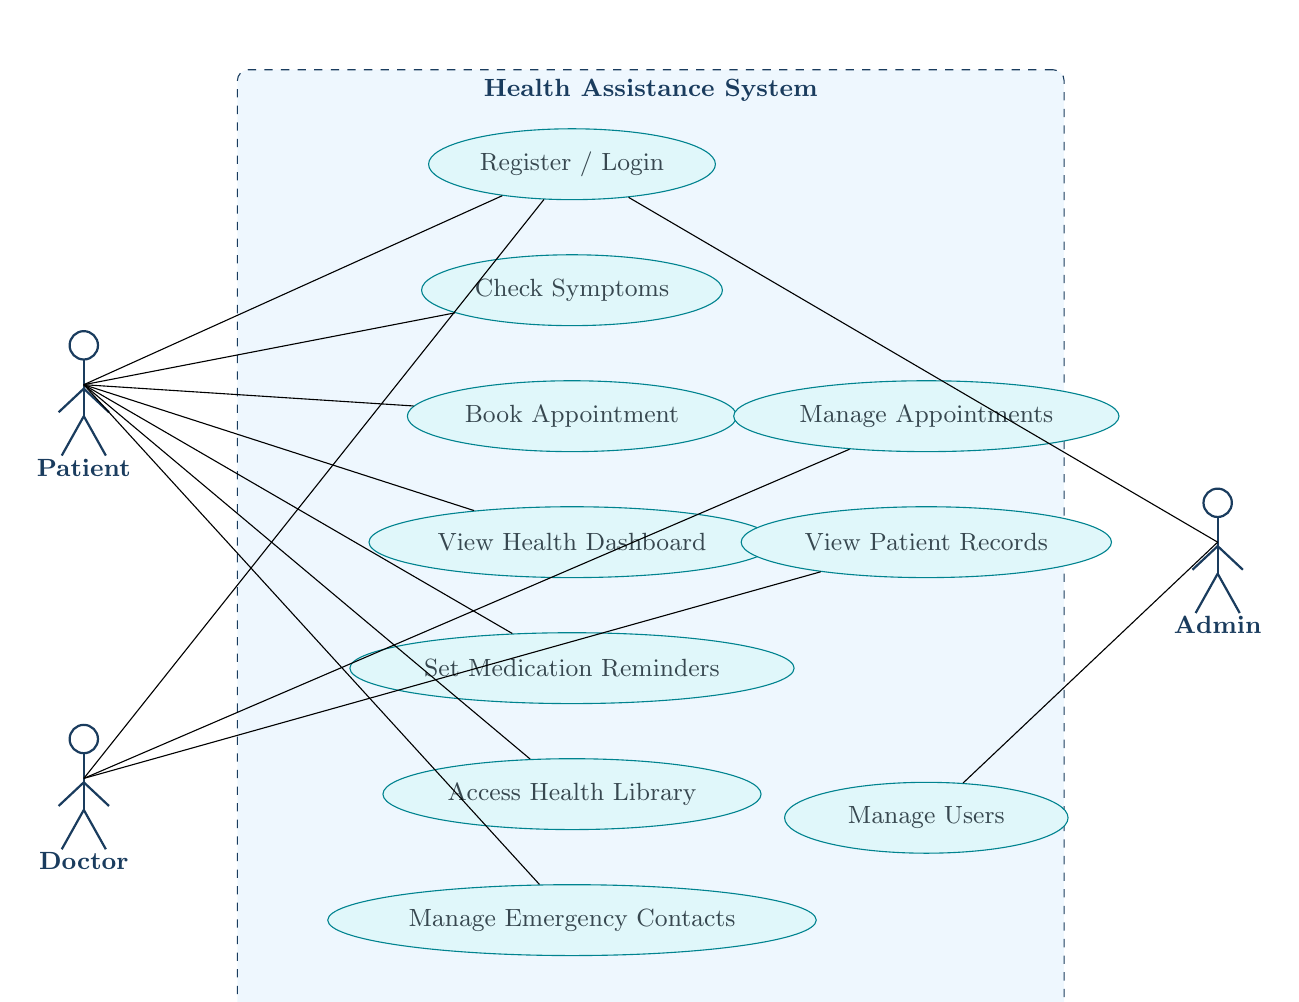
\begin{tikzpicture}[
  actor/.style={font=\small\bfseries, text=PrimaryBlue},
  usecase/.style={ellipse, draw=AccentTeal, fill=LightTeal,
    text=DarkGray, font=\small, align=center, minimum width=3.6cm,
    minimum height=0.9cm},
  sys/.style={rectangle, draw=PrimaryBlue, fill=LightBlue!60,
    rounded corners=4pt, dashed, inner sep=10pt}
]

% System boundary
\node[sys, minimum width=10.5cm, minimum height=12cm] (system) at (6,0) {};
\node[font=\bfseries\small\color{PrimaryBlue}, anchor=north] at (system.north)
  {Health Assistance System};

% Actors (drawn as small stick-figure icons for clarity)
\coordinate (patient) at (-1.2,2);
\begin{scope}[shift={(patient)}]
  \draw[PrimaryBlue, line width=0.8pt] (0,0.5) circle (0.18);
  \draw[PrimaryBlue, line width=0.8pt] (0,0.32) -- (0,-0.4);
  \draw[PrimaryBlue, line width=0.8pt] (0,-0.05) -- (-0.32,-0.35);
  \draw[PrimaryBlue, line width=0.8pt] (0,-0.05) -- (0.32,-0.35);
  \draw[PrimaryBlue, line width=0.8pt] (0,-0.4) -- (-0.28,-0.9);
  \draw[PrimaryBlue, line width=0.8pt] (0,-0.4) -- (0.28,-0.9);
  \node[font=\small, text=PrimaryBlue] at (0,-1.05) {\textbf{Patient}};
\end{scope}

\coordinate (doctor) at (-1.2,-3);
\begin{scope}[shift={(doctor)}]
  \draw[PrimaryBlue, line width=0.8pt] (0,0.5) circle (0.18);
  \draw[PrimaryBlue, line width=0.8pt] (0,0.32) -- (0,-0.4);
  \draw[PrimaryBlue, line width=0.8pt] (0,-0.05) -- (-0.32,-0.35);
  \draw[PrimaryBlue, line width=0.8pt] (0,-0.05) -- (0.32,-0.35);
  \draw[PrimaryBlue, line width=0.8pt] (0,-0.4) -- (-0.28,-0.9);
  \draw[PrimaryBlue, line width=0.8pt] (0,-0.4) -- (0.28,-0.9);
  \node[font=\small, text=PrimaryBlue] at (0,-1.05) {\textbf{Doctor}};
\end{scope}

\coordinate (admin) at (13.2,0);
\begin{scope}[shift={(admin)}]
  \draw[PrimaryBlue, line width=0.8pt] (0,0.5) circle (0.18);
  \draw[PrimaryBlue, line width=0.8pt] (0,0.32) -- (0,-0.4);
  \draw[PrimaryBlue, line width=0.8pt] (0,-0.05) -- (-0.32,-0.35);
  \draw[PrimaryBlue, line width=0.8pt] (0,-0.05) -- (0.32,-0.35);
  \draw[PrimaryBlue, line width=0.8pt] (0,-0.4) -- (-0.28,-0.9);
  \draw[PrimaryBlue, line width=0.8pt] (0,-0.4) -- (0.28,-0.9);
  \node[font=\small, text=PrimaryBlue] at (0,-1.05) {\textbf{Admin}};
\end{scope}

% Use cases
\node[usecase] (uc1)  at (5, 4.8) {Register / Login};
\node[usecase] (uc2)  at (5, 3.2) {Check Symptoms};
\node[usecase] (uc3)  at (5, 1.6) {Book Appointment};
\node[usecase] (uc4)  at (5, 0.0) {View Health Dashboard};
\node[usecase] (uc5)  at (5,-1.6) {Set Medication Reminders};
\node[usecase] (uc6)  at (5,-3.2) {Access Health Library};
\node[usecase] (uc7)  at (5,-4.8) {Manage Emergency Contacts};
\node[usecase] (uc8)  at (9.5, 1.6) {Manage Appointments};
\node[usecase] (uc9)  at (9.5, 0.0) {View Patient Records};
\node[usecase] (uc10) at (9.5,-3.5) {Manage Users};

% Patient associations
\draw (patient) -- (uc1);
\draw (patient) -- (uc2);
\draw (patient) -- (uc3);
\draw (patient) -- (uc4);
\draw (patient) -- (uc5);
\draw (patient) -- (uc6);
\draw (patient) -- (uc7);

% Doctor associations
\draw (doctor) -- (uc8);
\draw (doctor) -- (uc9);
\draw (doctor) -- (uc1);

% Admin associations
\draw (admin) -- (uc10);
\draw (admin) -- (uc1);

\end{tikzpicture}
\caption{System Use Case Diagram}
\end{figure}

\subsection{Class Diagram}

\begin{figure}[H]
\centering
\resizebox{\textwidth}{!}{%
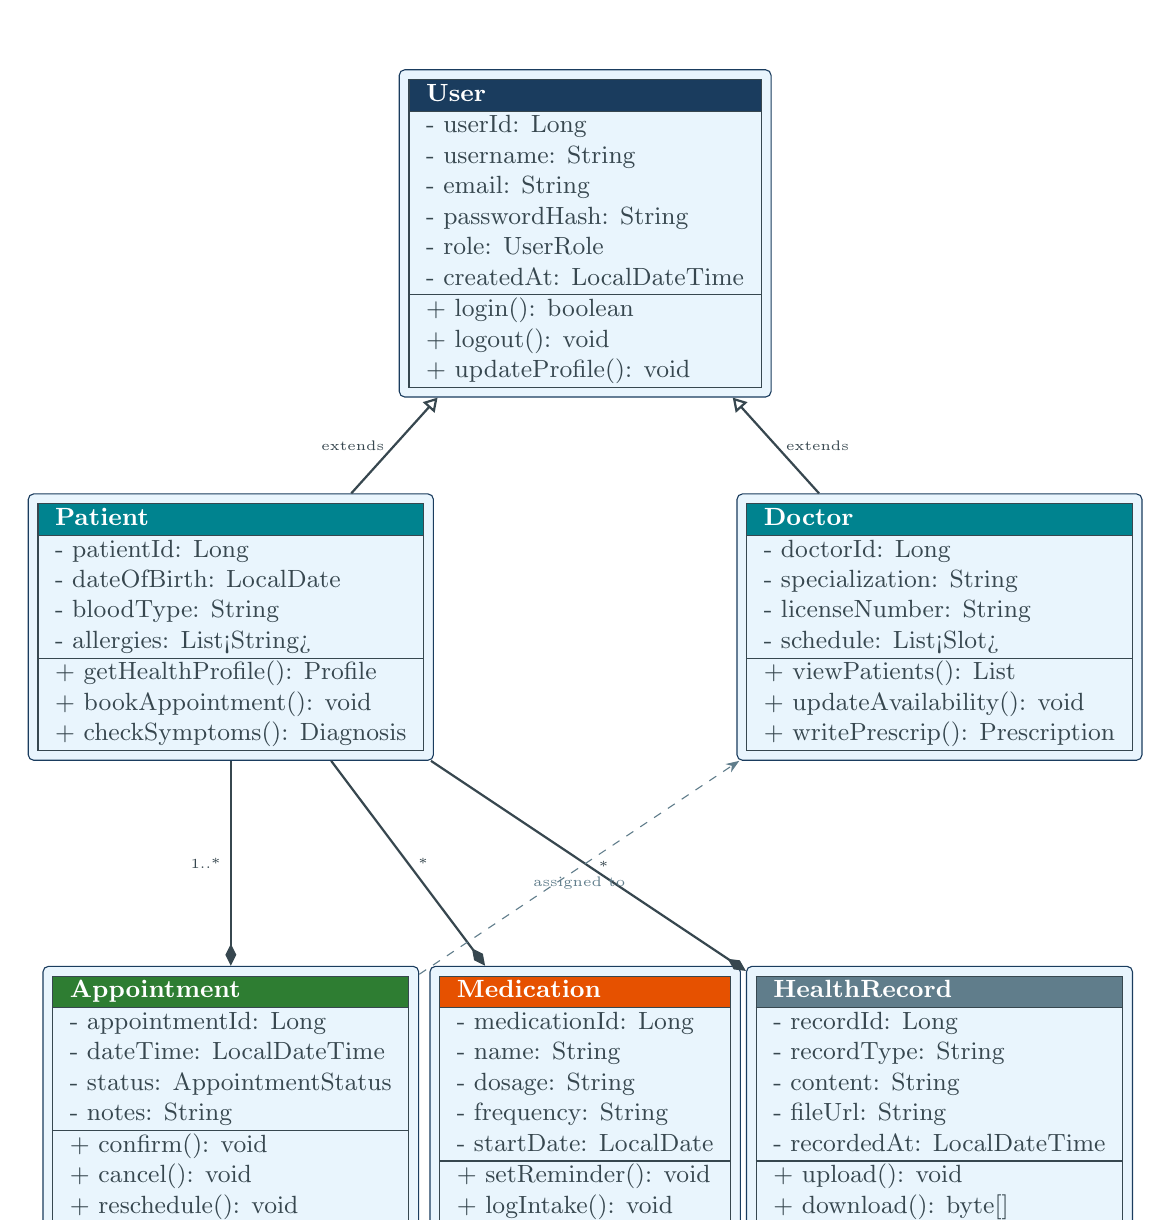
\begin{tikzpicture}[
  class/.style={rectangle, draw=PrimaryBlue, fill=LightBlue!80,
    rounded corners=2pt, font=\small, text=DarkGray},
  rel/.style={-{Triangle[open]}, thick, DarkGray},
  comp/.style={-{Diamond}, thick, DarkGray},
  dep/.style={dashed, -{Stealth}, MidGray}
]

% User class
\node[class] (user) at (0,0) {
  \begin{tabular}{|l|}
  \hline
  \rowcolor{PrimaryBlue}\color{White}\textbf{User} \\
  \hline
  - userId: Long \\
  - username: String \\
  - email: String \\
  - passwordHash: String \\
  - role: UserRole \\
  - createdAt: LocalDateTime \\
  \hline
  + login(): boolean \\
  + logout(): void \\
  + updateProfile(): void \\
  \hline
  \end{tabular}
};

% Patient class
\node[class] (patient) at (-4.5,-5) {
  \begin{tabular}{|l|}
  \hline
  \rowcolor{AccentTeal}\color{White}\textbf{Patient} \\
  \hline
  - patientId: Long \\
  - dateOfBirth: LocalDate \\
  - bloodType: String \\
  - allergies: List<String> \\
  \hline
  + getHealthProfile(): Profile \\
  + bookAppointment(): void \\
  + checkSymptoms(): Diagnosis \\
  \hline
  \end{tabular}
};

% Doctor class
\node[class] (doctor) at (4.5,-5) {
  \begin{tabular}{|l|}
  \hline
  \rowcolor{AccentTeal}\color{White}\textbf{Doctor} \\
  \hline
  - doctorId: Long \\
  - specialization: String \\
  - licenseNumber: String \\
  - schedule: List<Slot> \\
  \hline
  + viewPatients(): List \\
  + updateAvailability(): void \\
  + writePrescrip(): Prescription \\
  \hline
  \end{tabular}
};

% Appointment class
\node[class] (appt) at (-4.5,-11) {
  \begin{tabular}{|l|}
  \hline
  \rowcolor{AccentGreen}\color{White}\textbf{Appointment} \\
  \hline
  - appointmentId: Long \\
  - dateTime: LocalDateTime \\
  - status: AppointmentStatus \\
  - notes: String \\
  \hline
  + confirm(): void \\
  + cancel(): void \\
  + reschedule(): void \\
  \hline
  \end{tabular}
};

% Medication class
\node[class] (med) at (0,-11) {
  \begin{tabular}{|l|}
  \hline
  \rowcolor{WarnOrange}\color{White}\textbf{Medication} \\
  \hline
  - medicationId: Long \\
  - name: String \\
  - dosage: String \\
  - frequency: String \\
  - startDate: LocalDate \\
  \hline
  + setReminder(): void \\
  + logIntake(): void \\
  \hline
  \end{tabular}
};

% HealthRecord class
\node[class] (health) at (4.5,-11) {
  \begin{tabular}{|l|}
  \hline
  \rowcolor{MidGray}\color{White}\textbf{HealthRecord} \\
  \hline
  - recordId: Long \\
  - recordType: String \\
  - content: String \\
  - fileUrl: String \\
  - recordedAt: LocalDateTime \\
  \hline
  + upload(): void \\
  + download(): byte[] \\
  \hline
  \end{tabular}
};

% Relationships
\draw[rel] (patient) -- (user) node[midway, left, font=\tiny]{extends};
\draw[rel] (doctor) -- (user) node[midway, right, font=\tiny]{extends};
\draw[comp] (patient) -- (appt) node[midway, left, font=\tiny]{1..*};
\draw[comp] (patient) -- (med) node[midway, right, font=\tiny]{*};
\draw[comp] (patient) -- (health) node[midway, right, font=\tiny]{*};
\draw[dep] (appt) -- (doctor) node[midway, below, font=\tiny]{assigned to};

\end{tikzpicture}
}
\caption{System Class Diagram}
\end{figure}

%---------------------------------------------------------------
\subsection{Sequence Diagrams}
%---------------------------------------------------------------

\subsubsection{SD-1: User Registration and Login}

\begin{figure}[H]
\centering
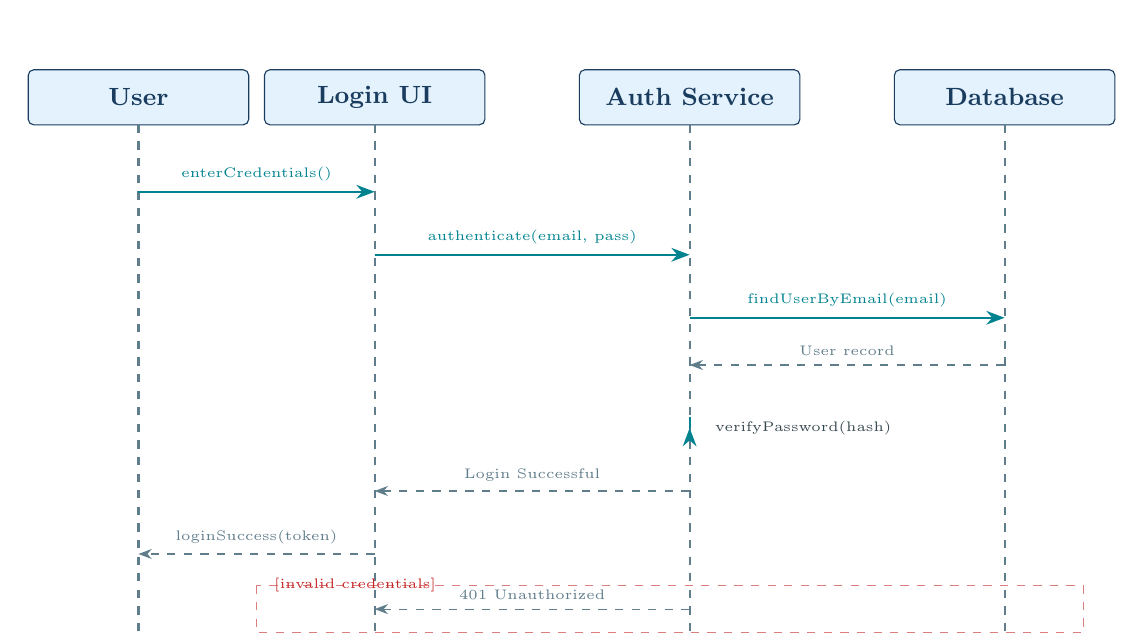
\begin{tikzpicture}[
  lifeline/.style={draw=MidGray, dashed, thick},
  obj/.style={rectangle, draw=PrimaryBlue, fill=LightBlue, rounded corners=2pt,
    font=\small\bfseries, minimum width=2.8cm, minimum height=0.7cm, text=PrimaryBlue},
  msg/.style={-{Stealth}, AccentTeal, thick},
  ret/.style={-{Stealth}, dashed, MidGray},
  act/.style={rectangle, fill=PrimaryBlue!25, draw=PrimaryBlue, minimum width=0.3cm}
]

\node[obj] (user)   at (0,0)   {User};
\node[obj] (ui)     at (3,0)   {Login UI};
\node[obj] (auth)   at (7,0)   {Auth Service};
\node[obj] (db)     at (11,0)  {Database};

\draw[lifeline] (0,-0.35)   -- (0,-7);
\draw[lifeline] (3,-0.35)   -- (3,-7);
\draw[lifeline] (7,-0.35)   -- (7,-7);
\draw[lifeline] (11,-0.35)  -- (11,-7);

% Messages
\draw[msg] (0,-1.2) -- (3,-1.2) node[midway,above,font=\tiny]{enterCredentials()};
\draw[msg] (3,-2.0) -- (7,-2.0) node[midway,above,font=\tiny]{authenticate(email, pass)};
\draw[msg] (7,-2.8) -- (11,-2.8) node[midway,above,font=\tiny]{findUserByEmail(email)};
\draw[ret] (11,-3.4) -- (7,-3.4) node[midway,above,font=\tiny]{User record};
\draw[msg] (7,-4.2) -- (7,-4.2);
\node[font=\tiny\color{DarkGray}, anchor=west] at (7.2,-4.2) {verifyPassword(hash)};
\draw[ret] (7,-5.0) -- (3,-5.0) node[midway,above,font=\tiny]{Login Successful};
\draw[ret] (3,-5.8) -- (0,-5.8) node[midway,above,font=\tiny]{loginSuccess(token)};

% Alt fragment
\draw[dashed, AlertRed!60] (1.5,-6.2) rectangle (12,-6.8);
\node[font=\tiny\color{AlertRed}, anchor=west] at (1.6,-6.2) {[invalid credentials]};
\draw[ret] (7,-6.5) -- (3,-6.5) node[midway,above,font=\tiny]{401 Unauthorized};

\end{tikzpicture}
\caption{SD-1: User Authentication Sequence}
\end{figure}

%---------------------------------------------------------------
\section{Technology Stack}
%---------------------------------------------------------------

\begin{table}[H]
\centering
\caption{Technology Stack}
\begin{tabularx}{\textwidth}{l l X}
\toprule
\rowcolor{PrimaryBlue!15}
\textbf{Layer} & \textbf{Technology} & \textbf{Purpose} \\
\midrule
\rowO UI & JavaFX, FXML, CSS & Desktop screens, layout, and styling \\
Logic & Java Controllers & User actions, validation, and screen flow \\
\rowO Data Access & JDBC / DAO classes & Database queries and persistence \\
Database & MySQL 8 & Persistent relational data storage \\
\rowO Background Tasks & Java threads / Platform.runLater & Appointment reminders and alerts \\
Build / Run & Java compiler and JavaFX SDK & Compile and launch the desktop application \\
\rowO Version Control & Git + GitHub & Source code management and collaboration \\
Project Mgmt & Team coordination & Agile sprint and task management \\
\bottomrule
\end{tabularx}
\end{table}

%===============================================================
% CHAPTER 4 -- RESULTS AND DISCUSSION
%===============================================================
\chapter{Results and Discussion}

\section{Application Screenshots}

This section presents screenshots of the Health Assistance System across its key functional areas. Replace each placeholder with the actual application screenshots.

\subsection{Authentication Screens}

\begin{figure}[H]
\centering
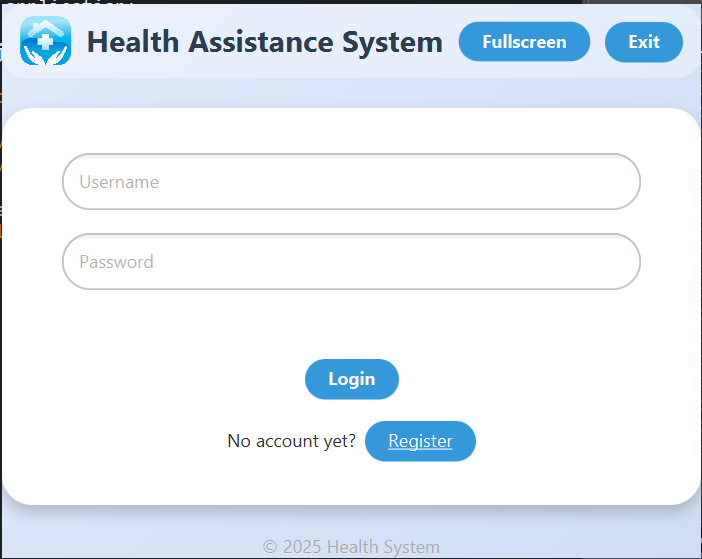
\includegraphics[width=0.6\textwidth]{assets/login.png}
\caption{Login Screen -- User authentication with email/password fields and role-based login}
\end{figure}

\begin{figure}[H]
\centering
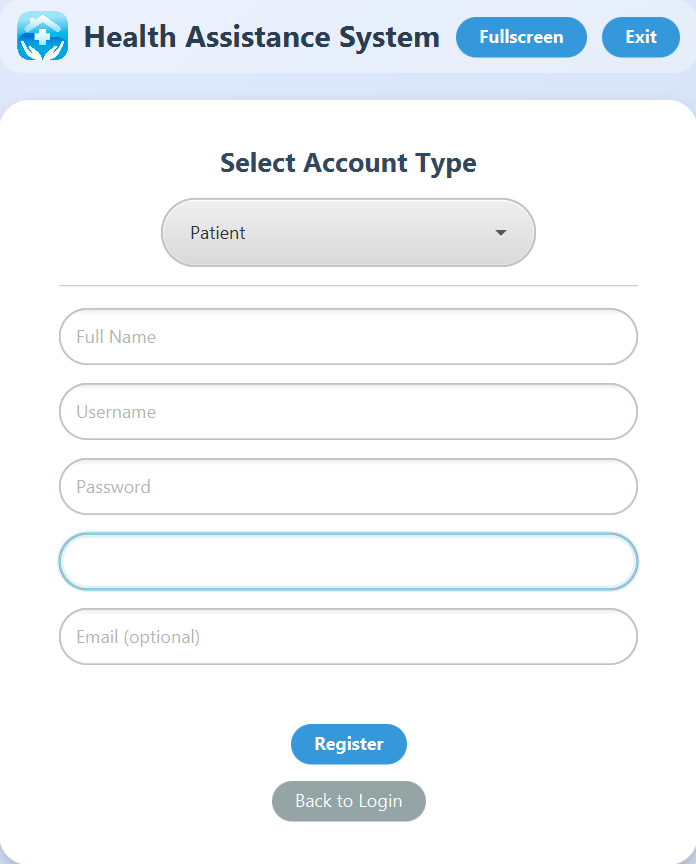
\includegraphics[width=0.6\textwidth]{assets/registration.png}
\caption{Registration Screen -- New user registration with field validation and role selection}
\end{figure}

\subsection{Patient Dashboard}

\begin{figure}[H]
\centering
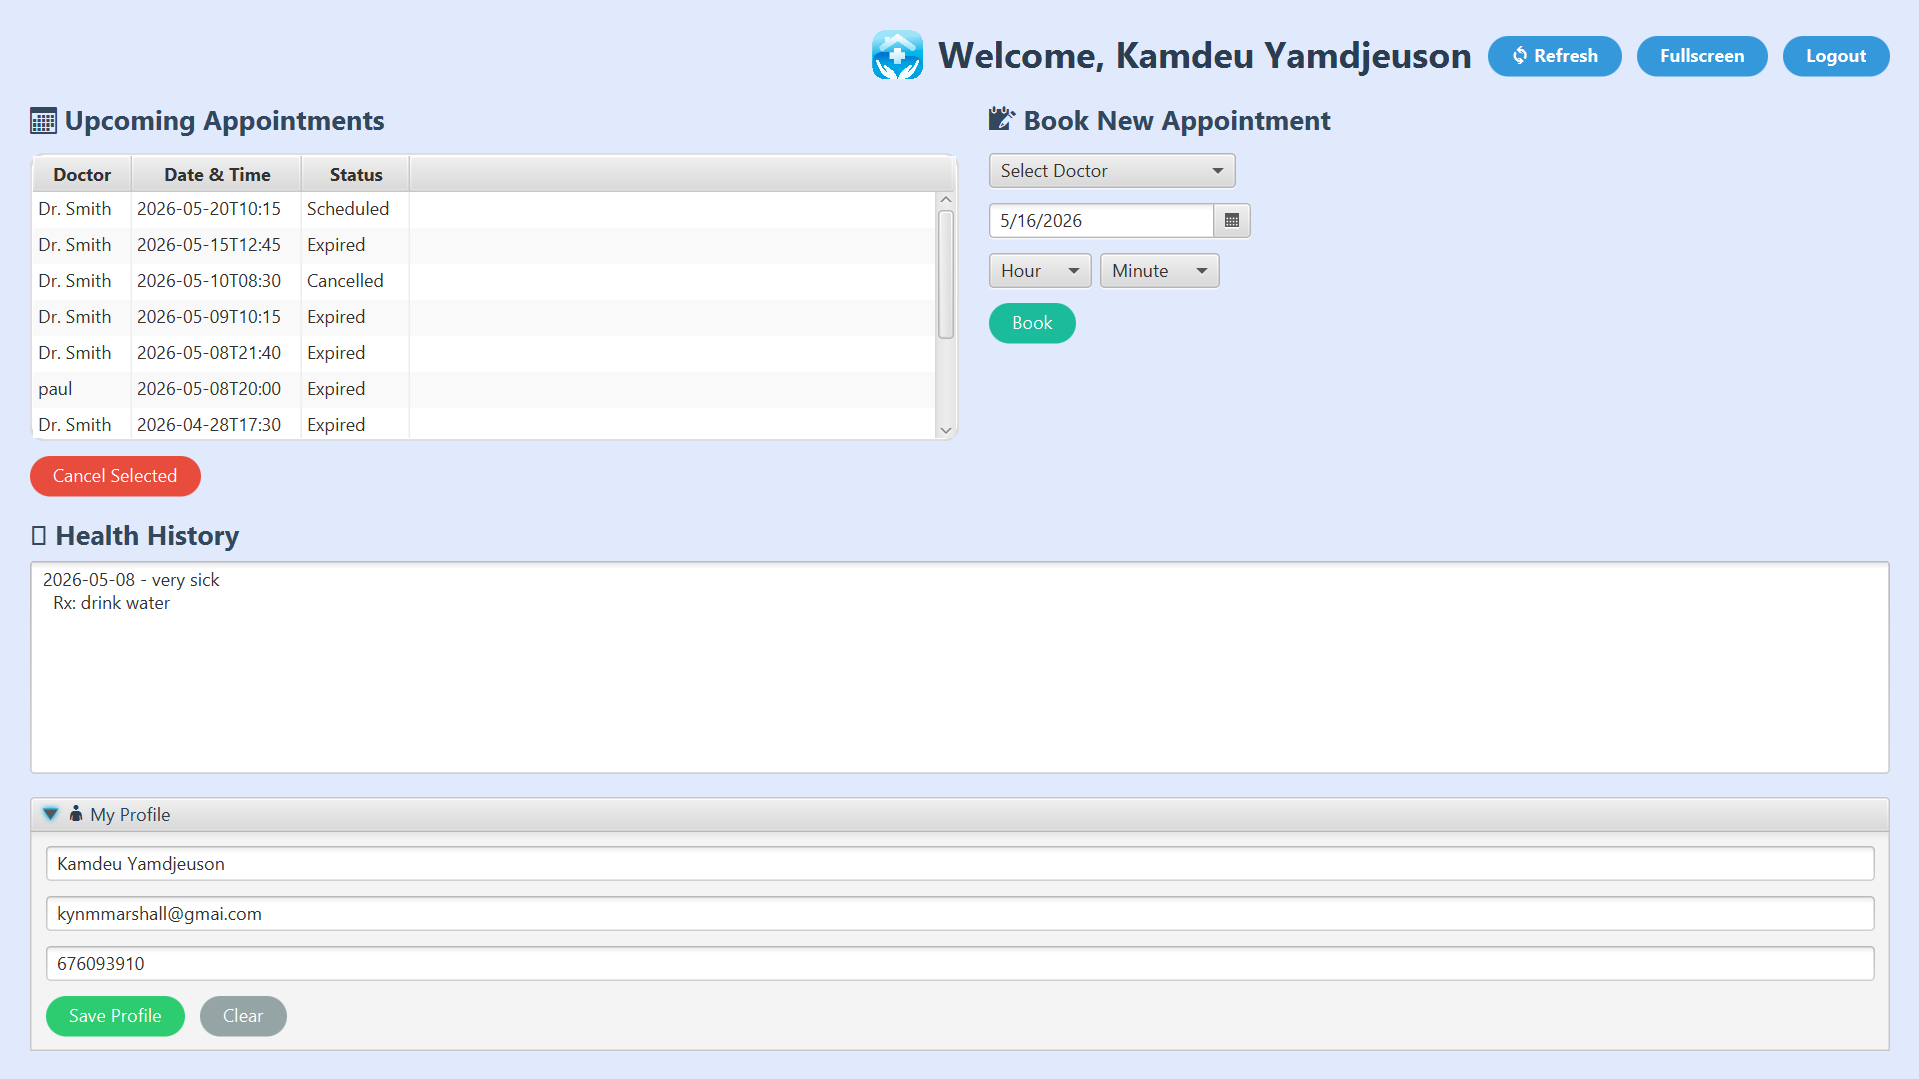
\includegraphics[width=0.85\textwidth]{assets/patientDashboard.png}
\caption{Patient Health Dashboard -- Overview of health metrics, appointments, medications, and alerts}
\end{figure}


\subsection{Doctor Portal}

\begin{figure}[H]
\centering
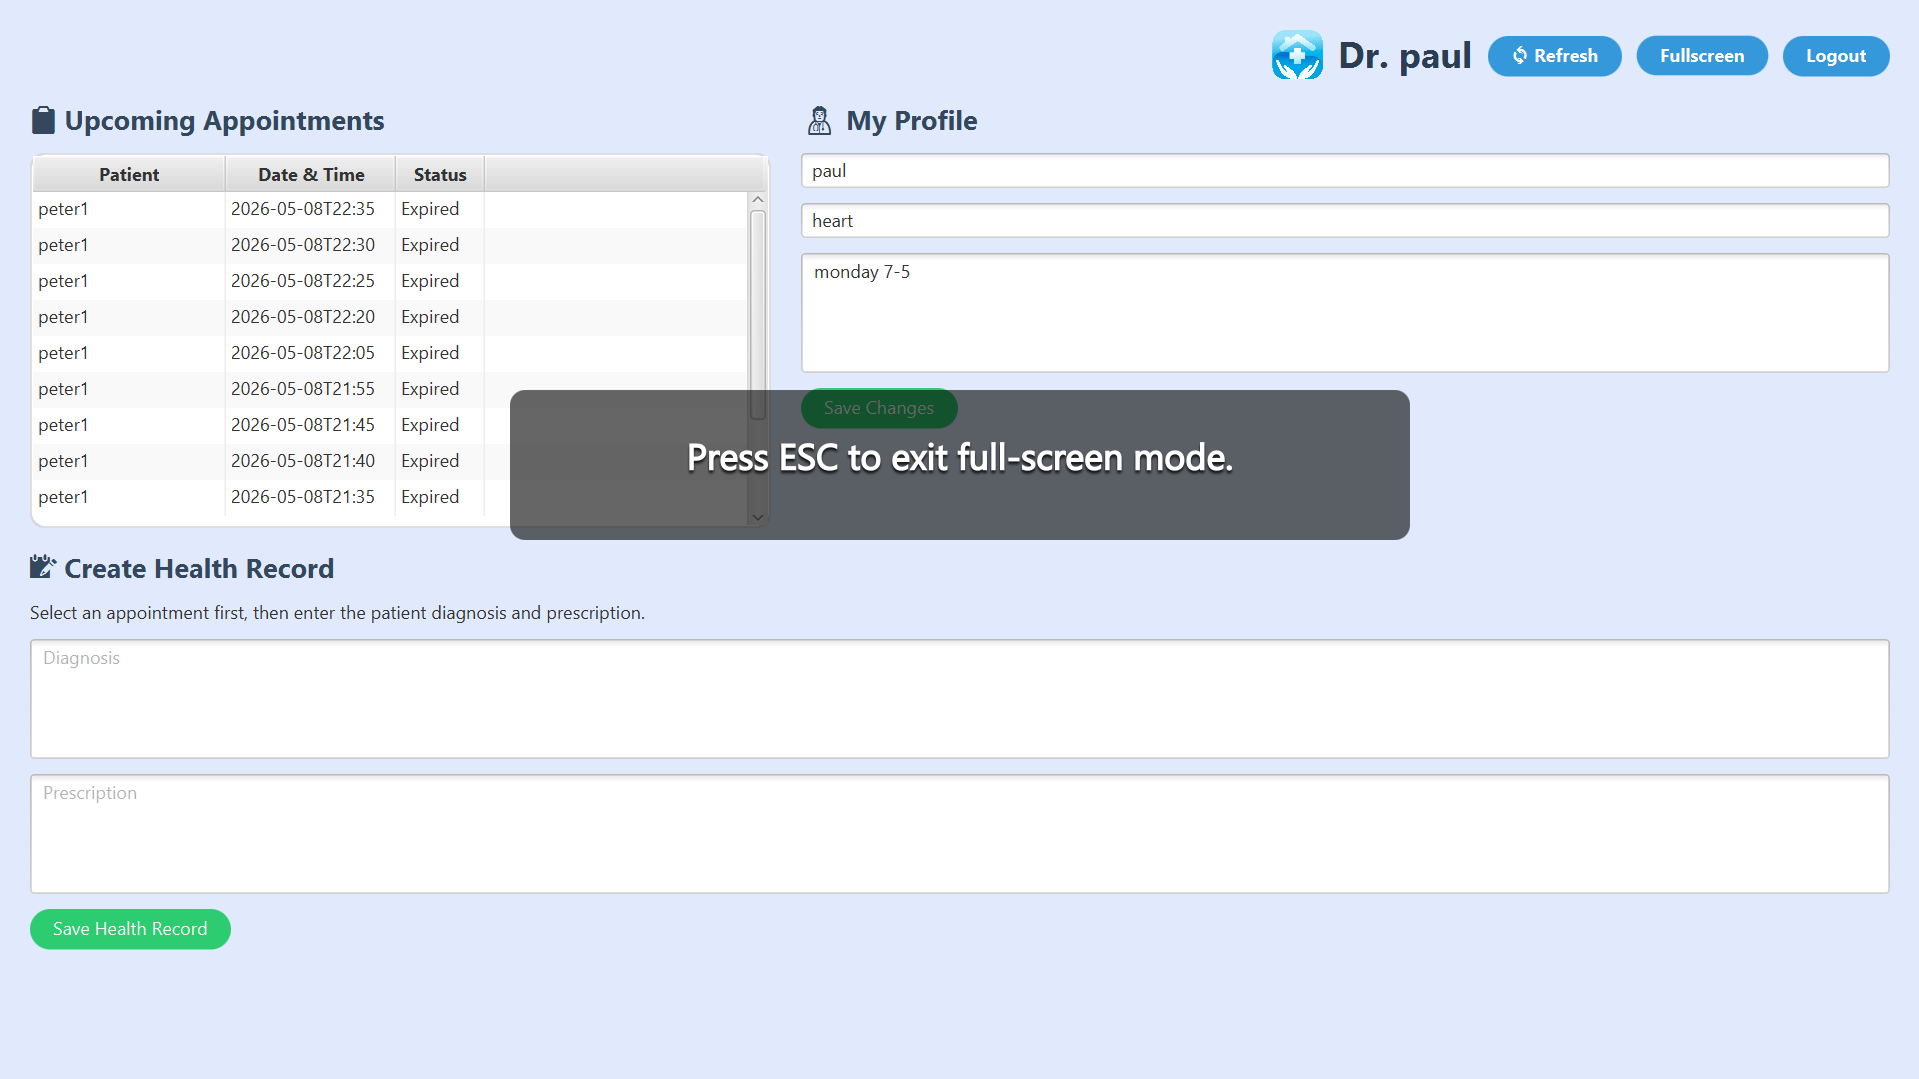
\includegraphics[width=0.85\textwidth]{assets/doctorDashboard.png}
\caption{Doctor Dashboard -- Schedule management, patient records, and clinical overview}
\end{figure}

\subsection{Admin Dashboard}

\begin{figure}[H]
\centering
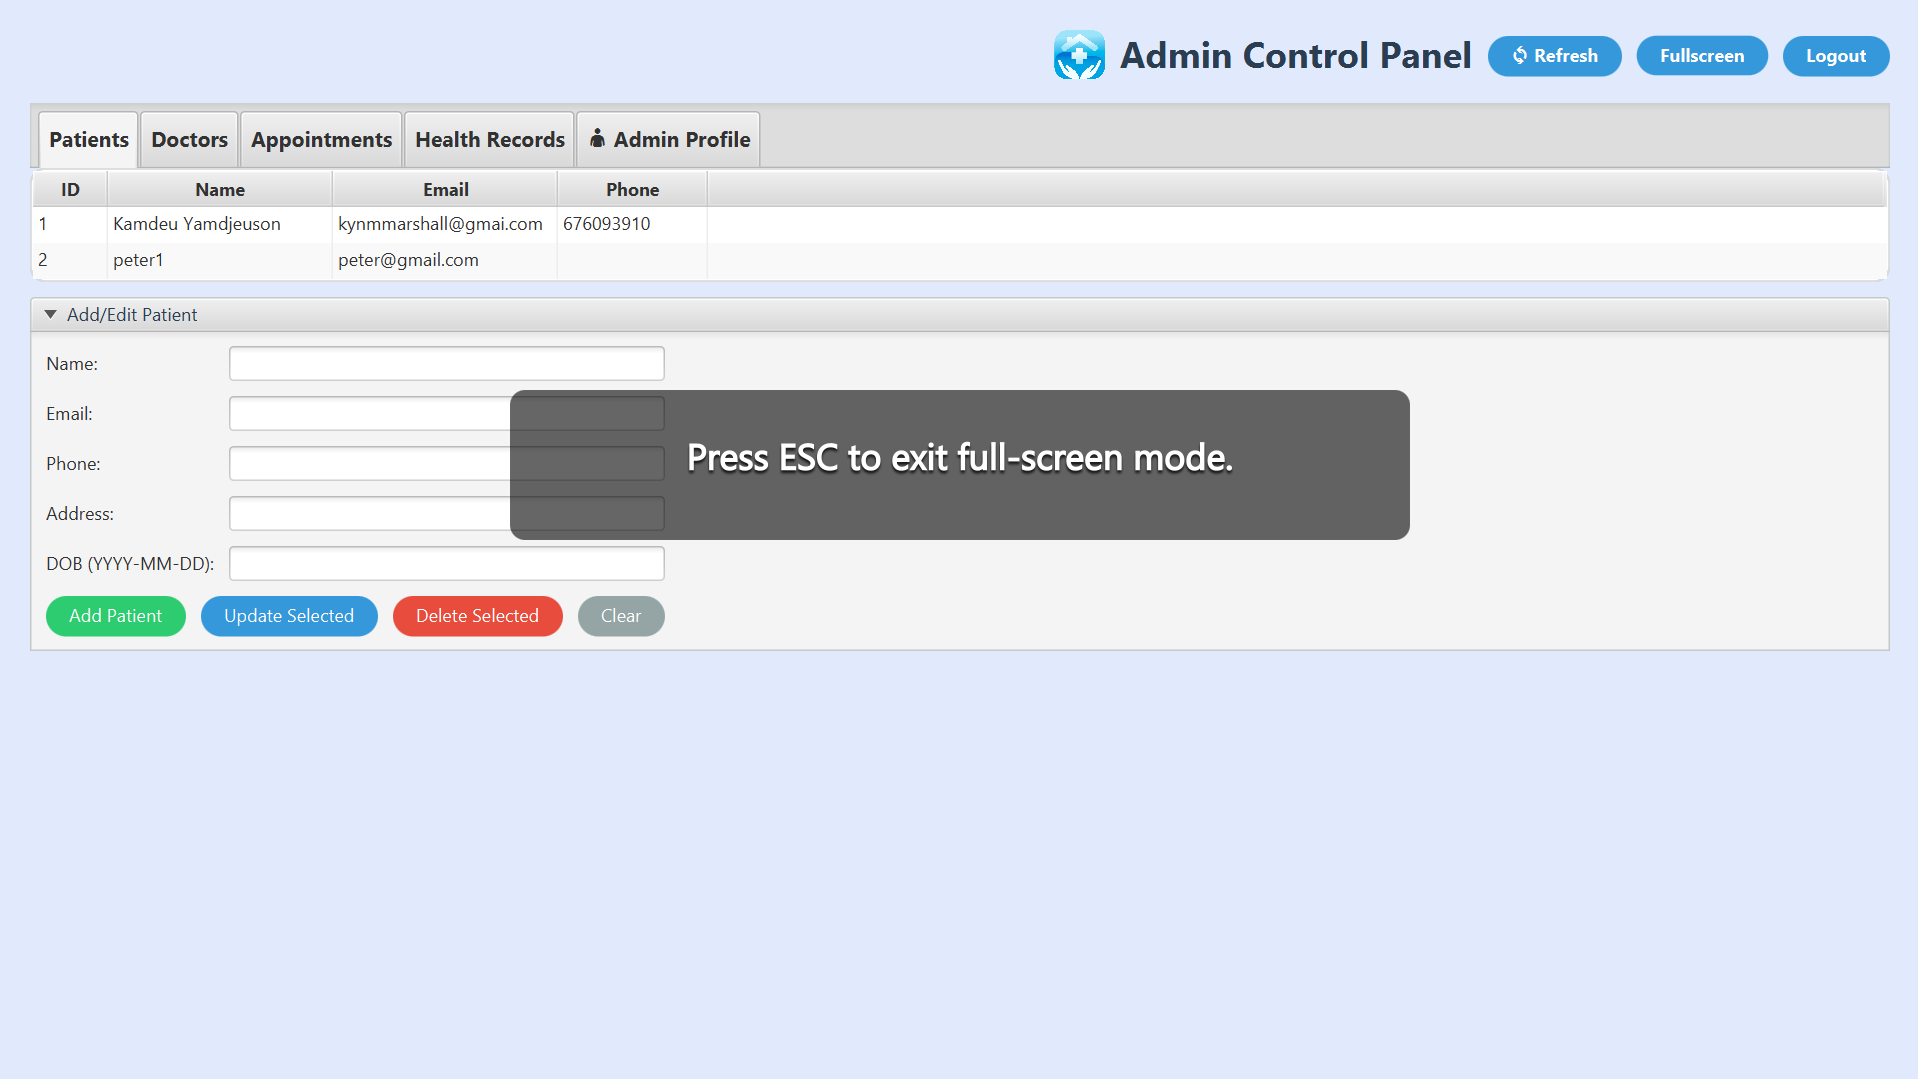
\includegraphics[width=0.85\textwidth]{assets/adminDashboard.png}
\caption{Admin Dashboard -- System management, user administration, and analytics}
\end{figure}

%===============================================================
% CHAPTER 5 -- CONCLUSION AND FUTURE WORK
%===============================================================
\chapter{Conclusion and Future Work}

\section{Summary of Project Outcomes}

The Health Assistance System successfully delivers a comprehensive, community-focused digital health platform built on solid software engineering principles. All six project phases were completed as scheduled within the Scrum framework, producing a functional application that addresses real-world health management challenges.

\begin{tcolorbox}[successbox, title={Key Achievements}]
\begin{itemize}[leftmargin=1.2cm]
  \item Fully functional JavaFX desktop application with role-based login
  \item Patient, doctor, and admin dashboards with persistent database-backed data
  \item Appointment booking system with conflict checking and expiration handling
  \item Automated appointment reminder with popup alert and looping sound
  \item Health record and profile management through DAO-based persistence
  \item Complete UML documentation (use cases, class, 5 sequence, 3 activity, deployment)
\end{itemize}
\end{tcolorbox}

\section{Challenges and Solutions}

\subsection{Technical Challenges}

\begin{itemize}[leftmargin=1.5cm]
  \item \textbf{Appointment Persistence:} Keeping appointment booking and status changes consistent required using DAO methods with validation and conflict checks.
  \item \textbf{Real-time Notifications:} Scheduling background reminder checks required a daemon thread and safe JavaFX UI updates with \texttt{Platform.runLater()}.
  \item \textbf{Database Consistency:} Time-based status updates had to be handled carefully so appointments were not marked expired too early.
\end{itemize}

\subsection{Collaboration Challenges}

\begin{itemize}[leftmargin=1.5cm]
  \item Coordinating concurrent development on shared modules led to merge conflicts, resolved by adopting a strict feature-branch Git workflow.
  \item Differing opinions on UI design were resolved through wireframe prototyping and feedback sessions.
\end{itemize}

\section{Lessons Learned}

\begin{enumerate}[leftmargin=1.5cm]
  \item Clear separation between controller, DAO, and model code makes debugging much easier in a JavaFX project.
  \item Scrum ceremonies, though brief, significantly improved team alignment and early identification of blockers.
  \item Database time handling is critical; application-side timestamps are more reliable than assuming database time matches local time.
  \item UML diagrams produced before coding, not after, genuinely guided implementation decisions.
\end{enumerate}

\chapter{Project Structure}

The project is organised as a JavaFX desktop application with source code, compiled output, and documentation:

\begin{lstlisting}[language=bash, caption={Project Directory Structure}]
HealthAssistanceSystem/
|---- src/
|   |---- application/
|   |---- controller/
|   |---- dao/
|   |---- database/
|   |---- model/
|   |---- resources/
|   |   |---- css/
|   |   '---- fxml/
|   '---- util/
|---- bin/
|---- Documentation/
|---- build.fxbuild
\end{lstlisting}

\end{document}